\documentclass[multi=page, border=2mm,tikz]{standalone}
\usepackage{tikz}
\usetikzlibrary{datavisualization}
\usetikzlibrary{datavisualization.formats.functions}
\pgfkeys{
    /pgf/number format/.cd, use comma, set thousands separator={\,},
}

% arara: pdflatex
% arara: latexmk: { clean: partial }
\begin{document}

% NOTE nome originale: plot-0 -> page=1
\begin{page}
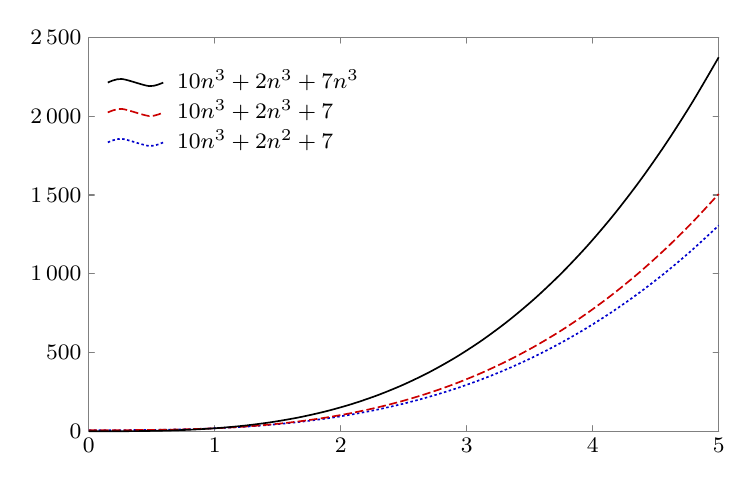
\begin{tikzpicture}
    \datavisualization [scientific axes=inner ticks,
                        legend={north west inside},
                        style sheet=strong colors,
                        style sheet=vary dashing,
                        x axis={length=8cm, min value=0, max value=5},
                        y axis={length=5cm, min value=0, max value=2500},
                        data/format=function,
                        visualize as smooth line/.list={omicron,theta,omega},
                        omicron={label in legend={text=$10n^3 + 2n^3 + 7n^3$}},
                        theta={label in legend={text=$10n^3 + 2n^3 + 7$}},
                        omega={label in legend={text=$10n^3 + 2n^2 + 7$}},
                        ]
    data [set=omicron] {
        var x : interval [0:5];
        func y = 10*\value x^3 + 2*\value x^3 + 7*\value x^3;
    }
    data [set=theta] {
        var x : interval [0:5];
        func y = 10*\value x^3 + 2*\value x^3 + 7;
    }
    data [set=omega] {
        var x : interval [0:5];
        func y = 10*\value x^3 + 2*\value x^2 + 7;
    };
\end{tikzpicture}
\end{page}

% NOTE nome originale: plot-0bis -> page=2
\begin{page}
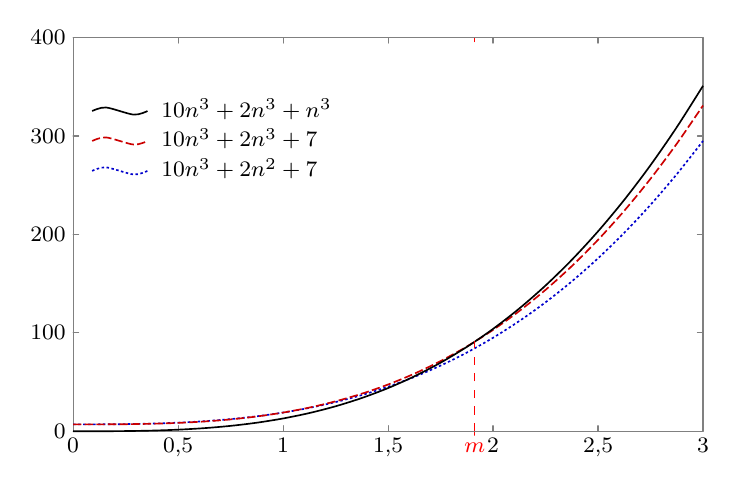
\begin{tikzpicture}
    \datavisualization [scientific axes=inner ticks,
                        legend={north west inside},
                        style sheet=strong colors,
                        style sheet=vary dashing,
                        x axis={length=8cm, min value=0, max value=3, ticks={some, major also at={1.9129 as [{style=red, low=-0.05cm}] $m$}}},
                        y axis={length=5cm, min value=0, max value=400},
                        data/format=function,
                        visualize as smooth line/.list={omicron,theta,omega},
                        omicron={label in legend={text=$10n^3 + 2n^3 + n^3$}},
                        theta={label in legend={text=$10n^3 + 2n^3 + 7$}},
                        omega={label in legend={text=$10n^3 + 2n^2 + 7$}},
                        ]
    data [set=omicron] {
        var x : interval [0:3];
        func y = 10*\value x^3 + 2*\value x^3 + \value x^3;
    }
    data [set=theta] {
        var x : interval [0:3];
        func y = 10*\value x^3 + 2*\value x^3 + 7;
    }
    data [set=omega] {
        var x : interval [0:3];
        func y = 10*\value x^3 + 2*\value x^2 + 7;
    };
    \draw [dashed, red] (5.1005,0) -- (5.1005,1.15);
\end{tikzpicture}
\end{page}

% NOTE nome originale: plot-1 -> page=2
\begin{page}
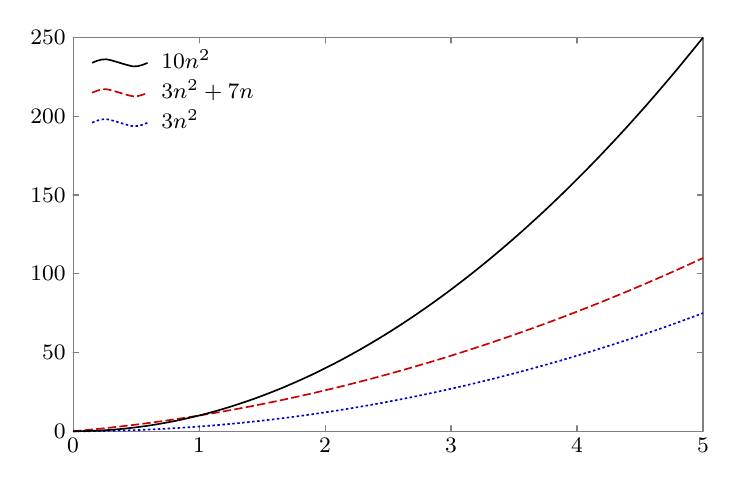
\begin{tikzpicture}
    \datavisualization [scientific axes=inner ticks,
                        legend={north west inside},
                        style sheet=strong colors,
                        style sheet=vary dashing,
                        x axis={length=8cm, min value=0, max value=5},
                        y axis={length=5cm, min value=0, max value=250},
                        data/format=function,
                        visualize as smooth line/.list={omicron,theta,omega},
                        omicron={label in legend={text=$10n^2$}},
                        theta={label in legend={text=$3n^2 + 7n$}},
                        omega={label in legend={text=$3n^2$}},
                        ]
    data [set=omicron] {
        var x : interval [0:5];
        func y = 10*\value x^2;
    }
    data [set=theta] {
        var x : interval [0:5];
        func y = 3*\value x^2 + 7*\value x;
    }
    data [set=omega] {
        var x : interval [0:5];
        func y = 3*\value x^2;
    };
\end{tikzpicture}
\end{page}

% NOTE nome originale: plot-2 -> page=3
\begin{page}
\def\mytypesetter#1{%
    \pgfmathparse{#1/pi}%
    \pgfmathprintnumber{\pgfmathresult}$\pi$%
}

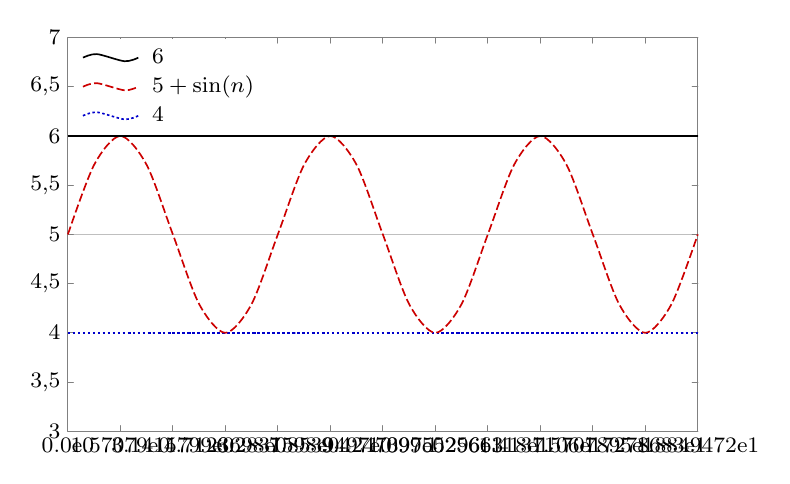
\begin{tikzpicture}
    \datavisualization [scientific axes=inner ticks,
                        legend={at values={x=3, y=6.5}},
                        style sheet=strong colors,
                        style sheet=vary dashing,
                        x axis={length=8cm, min value=0, max value=18.8495559215, ticks={step=(0.5*pi), tick typesetter/.code=\mytypesetter{##1}}},
                        y axis={length=5cm, min value=3, max value=7, ticks={step=0.5}, grid={ major also at={(5)} }},
                        data/format=function,
                        visualize as smooth line/.list={omicron,sine,omega},
                        omicron={label in legend={text=$6$}},
                        sine={label in legend={text=$5 + \sin(n)$}},
                        omega={label in legend={text=$4$}},
                        ]
    data [set=omicron] {
        var x : interval [0:2*pi*3];
        func y = 6;
    }
    data [set=sine] {
        var x : interval [0:2*pi*3];
        func y = 5 + sin(\value x r);
    }
    data [set=omega] {
        var x : interval [0:2*pi*3];
        func y = 4;
    };
\end{tikzpicture}
\end{page}

% NOTE nome originale: plot-3 -> page=4
\begin{page}
\begin{tikzpicture}

\end{tikzpicture}
\end{page}

% NOTE nome originale: plot-nvsn -> page=5
\begin{page}
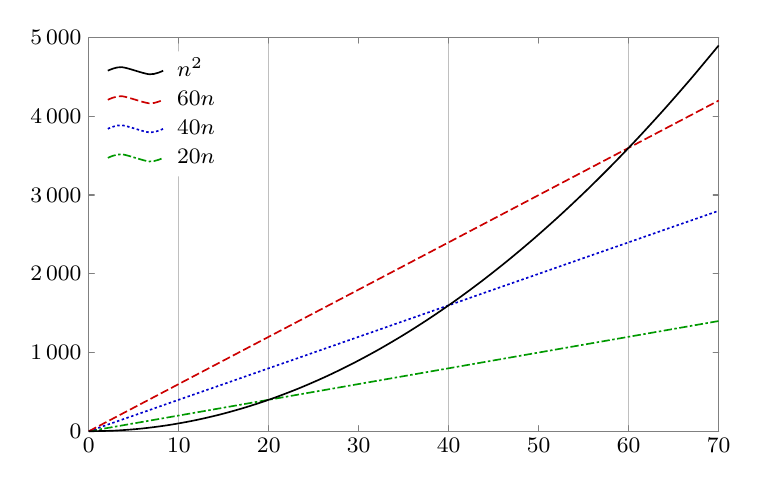
\begin{tikzpicture}
    \datavisualization [scientific axes=inner ticks,
                        legend={north west inside},
                        style sheet=strong colors,
                        style sheet=vary dashing,
                        x axis={length=8cm, min value=0, max value=70, grid={major also at={10,20,40,60}}},
                        y axis={length=5cm, min value=0, max value=5000},
                        data/format=function,
                        visualize as smooth line/.list={main,omicron,theta,omega},
                        main={label in legend={text=$n^2$}},
                        omicron={label in legend={text=$60n$}},
                        theta={label in legend={text=$40n$}},
                        omega={label in legend={text=$20n$}},
                        ]
    data [set=main] {
        var x : interval [0:70];
        func y = \value x^2;
    }
    data [set=omicron] {
        var x : interval [0:70];
        func y = 60*\value x;
    }
    data [set=theta] {
        var x : interval [0:70];
        func y = 40*\value x;
    }
    data [set=omega] {
        var x : interval [0:70];
        func y = 20*\value x;
    };
\end{tikzpicture}
\end{page}

\end{document}